\documentclass[a4paper,12pt]{report}

\usepackage[utf8]{inputenc}
\usepackage[T1]{fontenc}
\usepackage[english]{babel}
\usepackage{fullpage}
\usepackage{amsmath, amsfonts, amsthm}
\usepackage{latexsym, amssymb, mathrsfs}
\usepackage{wasysym}
\usepackage{tabularx}
\usepackage{enumerate}
%\usepackage{tcolorbox}
%\usepackage[framed,numbered,autolinebreaks,useliterate]{mcode}
\usepackage{graphicx}
\usepackage{hyperref}
\usepackage{url}
%\usepackage{caption}
\usepackage{subcaption}
%\usetikzlibrary{calc}
\usepackage{natbib}
\usepackage{epstopdf}
\usepackage{hhline}
\usepackage{colortbl}

\bibliographystyle{plainnat}

\linespread{1.10}


%\date{\today}



\begin{document}

\begin{center}

% Oberer Teil der Titelseite:

\textsc{\LARGE TU WIEN}\\[1.5cm]

\textsc{\Large Exercise 3 Group 20}\\[0.4cm]


% Title
\thispagestyle{empty}
\newcommand{\HRule}{\rule{\linewidth}{0.5mm}}
\HRule \\[0.4cm]
{ \huge \bfseries Topic 3.1.3: backdoor/poisoning attacks and defenses}\\[0.3cm]

\HRule \\[1.2cm]
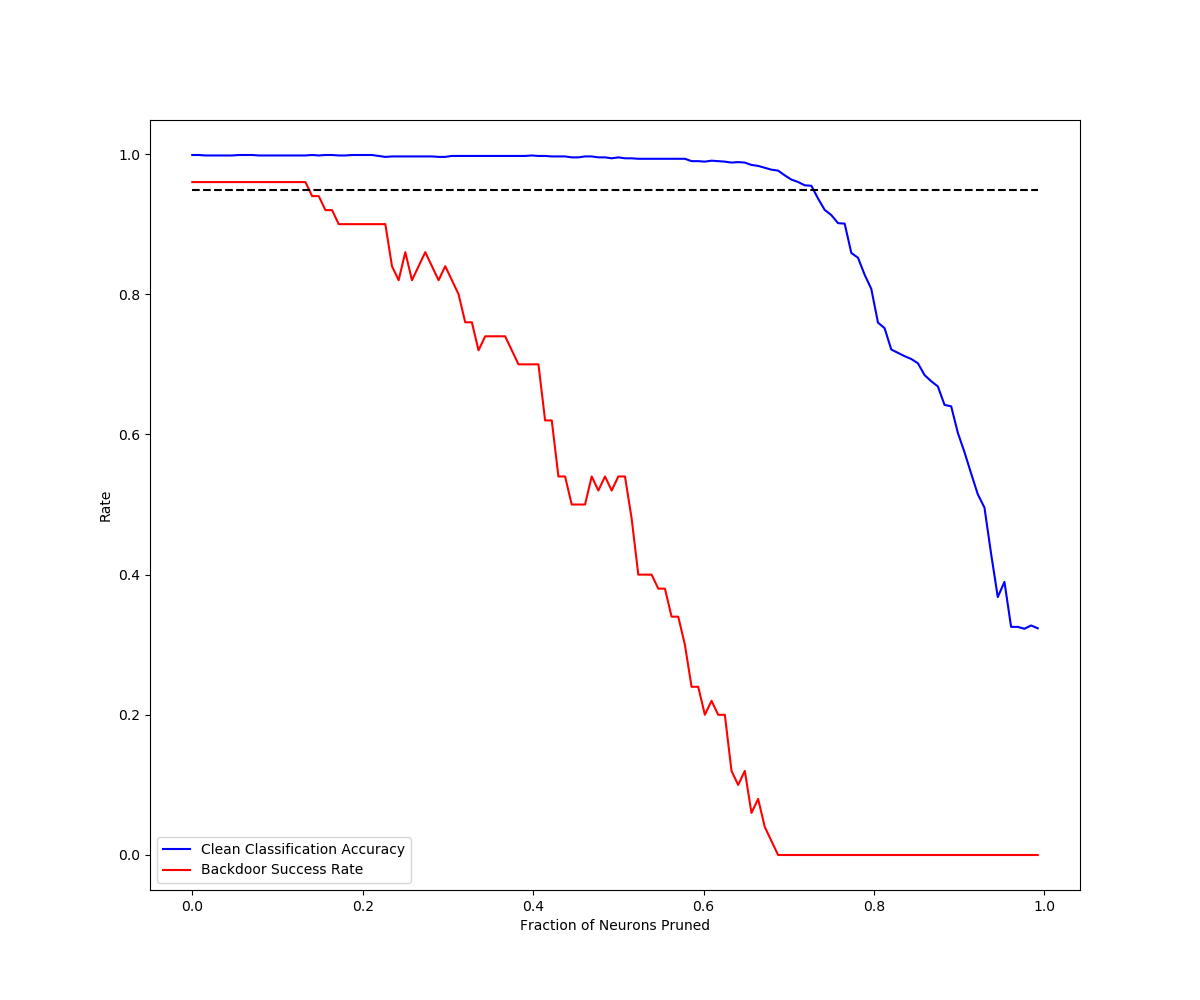
\includegraphics[width=0.65\textwidth]{./title}\\[0.5cm]

\Large{Wintersemester 2019/20}\\ [0.8cm]
\Large{184.702} \\ [0.3cm]

\begin{flushleft} \large
\emph{Autors:}\\
Sophie \textsc{Rain} 01425316,\\
Peter\textsc{Stroppa} 01326468,\\
 Lucas \textsc{Unterberger} 01325438 \\[0.5cm]
\end{flushleft}

% Unterer Teil der Seite
{\large \today}

\end{center}

\tableofcontents
\thispagestyle{empty}
\newpage
	
\chapter{Motivation}
Deep Learning, Artificial Intelligence and Neural Networks are words that you will hear quite often these days. Although the use of machine learning is not always necessary, to solve a problem, there is currently a huge trend using it as often as possible. Even though they might not be the cure for all our problems, Neural Networks are quite powerful and give way to some advanced technologies. One of them being image recognition. A Convolutional Neural Network refer to chapter[\ref{CNN}] for closer information, can easily classify previously unseen images into one of several predefined classes. Those networks, whilst being quite powerful come unfortunately with one big drawback. Even though computational power is ever increasing, training a Deep Neural Network might take from several hours up to multiple days. How long it actually takes, to fully train your network depends a lot on the chosen architecture and the input of the Neural Network. Therefore many companies opt to outsource model training to a third party. This third party then returns a trained model which the company can use for classification purposes. While Outscoring to a competent partner might seem like a reasonable thing to do, it opens doors for malicious people, to attack your network. One possible attack is called Backdoor/poisoning Attack. 
Backdoor Attacks belong to the class of training-time attacks, which means that an untrustworthy party intents to embed hidden information within the returned model during training. The model should classify normally on the test and validation data, but should misclassify on a certain set of 'poisoned' data. 'Poisoned' in this case means that there is some kind of trigger embedded in the picture.
Let's explain this attack in a more practical way. A government orders a private company to develop and train a Neural Network, so that it can be used for face recognition. That company does deliver the ordered Neural Network but has implemented a backdoor within it. I.e. if the face of any employee is checked, the person would be classified as somebody else if she wore green sunglasses on the photo.

\section{Introduction}
In this work we briefly show how to implement a Convolutional Neural Network and a backdoor attack and then focus on defenses against them. Our work is based on \citep{paper}.
Convolutional neural networks (CNN)\label{CNN} are Deep Neural Networks i.e. networks that contain at least one hidden layer, that are sparse, (many of
their weights are zero) and structured, in such a way, that neuron outputs depend only on neighboring neurons from the previous layer. Generally backdoor attacks are possible because Neural Networks use too many neurons within the hidden layers. Therefore one can encode certain behavior within rarely used nodes. A natural defense against this attack is the Pruning Defense. The defender prunes certain neurons in the model and uses this model to classify new input. Since the backdoor was encoded on neurons with low average activation, after deleting them, the backdoor attack should be nullified. However if the attacker suspects the defender to employ this defense, he can alter his attack to a so-called Pruning-Aware Attack. This attack prunes the model before training, embeds the hidden information within the pruned model and then unprunes the model again. The Pruning Defense of the defender will thus be largely ineffective. The paper refers to a last defense method, the Fine-Pruning Defense, which is effective against the Pruning-Aware Attack and a viable line of defense against all other mentioned attacks. Basically it combines the Pruning Defense and Fine-tuning, which is a computationally inexpensive way of retraining the model a 'tiny bit'. In this work we try to recreate all of these attacks and defenses, in order to verify the stated conclusions. 

\section{Preliminaries}
We were given a set of train- and test-traffic signs and a set of poisoned train- and test-traffic signs. Our objective, was to launch a targeted backdoor attack against an image classification Neural Network. Then we should employ the previously mentioned defenses and attacks and evaluate their respective effectiveness.

We started by analyzing the given data. Upon further inspection we realized that the folder train-GoLeft contained no images at all. The corresponding test-folder was not empty. This lead to discussions whether to allow this class, since we had no train-images. Basically our algorithm would never be able to classify these images correctly on purpose. Therefore we decided to delete this folder entirely. This left us with 9 different classes, all of which had images in the train and test set. The poisoned images were exclusively stop signs and the targeted class was CanGoStraightAndTurn. Therefore we included the poisoned train-signs in the CanGoStraightAndTurn folder. For better handling the poisonous test folder was kept separate from the other test folders. Our model would therefore classify a poisoned stop sign during training as a CanGoStraightAndTurn sign and thus hopefully misclassify a poisoned test sign when predicting. 

We implemented a Convolutional Neural Network (CNN) commonly used for image recognition, instead of a Faster regional Convolutional Neural Network (F-RCNN), like in the paper. F-RCNN is a high-end image recognition algorithm, that extracts regions from images and is able to classify sub-images within these regions. It's based on three Machine Learning models, run in sequence. Therefore training with this algorithm would have exhausted our computational resources manifold. Since our given images contain only the traffic sign and no redundant information, we decided that a 'normal' CNN provides perfectly acceptable results.

Our code is written in python and we made heavy use of the keras package, a package based on tensorflow. We used an already existing CNN model as found in a blogpost of \citep{architecture}. We adapted his code, and used an improved preprocessing method, i.e. standardizing the histogram of all pictures. We also used the keras-surgeon package from \citep{surgeon} to implement the pruning defense.  Keras-surgeon amongst other things allows us to manually delete certain channels within a convolutional layer. The Fine-tuning method was implemented using standard Keras functionality. Fine pruning was achieved by applying first the pruning and afterwards the fine tuning function. Like in the paper the pruning aware attack was developed in four consecutive steps.


\chapter{Methods and Results}
We first constructed an image classification model, trained on the poisoned train-data. Our models architecture is found in the table below. It is a Sequential keras model, based on \citep{architecture}.
\section{the model}
\begin{center}
	Model: 'sequential$\_$1'
\begin{tabular}{|l l l l|}\hline
	\hline
	Layer (type)                  & Output Shape       & Parameters & Act\\ \hline \hline
	conv2d$\_$1 (Conv2D)             & (None, 32, 32, 32)    & 2432  & relu\\ \hline
%	                              &                    &        &\\ \hline
	batch$\_$normalization$\_$1 (Batch) & (None, 32, 32, 32)    & 128   &\\ \hline
%	&                    &       & \\ \hline 
	max$\_$pooling2d$\_$1 (MaxPooling2D) & (None, 16, 16, 32)    & 0   &\\ \hline
%	&                    &        &\\ \hline
	dropout$\_$1 (Dropout) & (None, 16, 16, 32)    & 0   &\\ \hline
%	&                    &       & \\ \hline
	conv2d$\_$2 (Conv2D)             & (None, 16, 16, 64)    & 51264   & relu\\ \hline
%	&                    &        &\\ \hline
	batch$\_$normalization$\_$2 (Batch) & (None, 16, 16, 64)    & 256  & \\ \hline
%	&                    &       & \\ \hline 
	conv2d$\_$3 (Conv2D) & (None, 16, 16, 128)    & 204928   & relu \\ \hline
%	&                    &        &\\ \hline
	batch$\_$normalization$\_$3 (Batch) & (None, 16, 16, 128)    & 512  & \\ \hline
%	&                    &       & \\ \hline
	max$\_$pooling2d$\_$2 (MaxPooling2D) & (None, 8, 8, 128)    & 0  & \\ \hline
%	&                    &        &\\ \hline
	dropout$\_$2 (Dropout) & (None, 8, 8, 128)    & 0   &\\ \hline
%	&                    &        &\\ \hline
	flatten$\_$1 (Flatten) & (None, 8192)    & 0   &\\ \hline
%	&                    &        &\\ \hline
	dense$\_$1 (Dense) & (None, 512)    & 4194816   & relu \\ \hline
%	&                    &       & \\ \hline
	batch$\_$normalization$\_$4 (Batch) & (None, 512)    & 2048   &\\ \hline
%	&                    &        &\\ \hline
	dropout$\_$3 (Dropout) & (None, 512)    & 0  & \\ \hline
%	&                    &       & \\ \hline
	dense$\_$2 (Dense) & (None, 9)    & 4617  & softmax\\ \hline \hline
	Total parameter: 4,461,001 & & & \\
	Trainable parameter: 4,459,529 & & & \\
	Non-trainable parameter: 1,472 & & & \\ \hline
\end{tabular} 
\end{center}
We trained this model for 100 epochs and managed to achieve high accuracy on the clean test-data and low accuracy on the poisoned test-data. Since Backdoor success = 1 - accuracy of poisoned test-data, we are very happy with our model and its architecture. 
\section{standard attack}

\section{defenses}
\subsection{pruning}
Next we considered the Pruning Defense. First we need to get the average activations of every channel within the last convolutional Layer, just like in the paper. Notice that in the last convolutional layer (conv2d$\_$3) the output for a single test instance has shape (1, 16, 16, 128). This means that every single picture has 128 (1 for each channel) $16 \times 16$ matrices as output. The activation of a channel is precisely the sum of all elements of its output matrix. The activation of a picture are 128 activations of the 128 output channels. The average activation of a set of pictures is then for every channel the average of those activations. We now start with our trained model and calculate the average activation for each channel and then iteratively remove channels with the lowest average activation. A defender does not what the poisoned images look like, so she will keep pruning the model, until a significant reduction of accuracy occurs. We assumed pruning continues until a 5$\%$ drop of accuracy occurs. For demonstartion purposes we pruned until the very last channel and plotted the results.
\\
--\\
Graphik hier!\\
--\\
As you can see the Pruning Defense is capable to reduce backdoor success rate by a tremendous amount. Although one can argue that the backdoor success rate is still too high, since for practical applications, a machine learning algorithm, with a backdoor success rate of anything above 5$\%$ is unusable in real life applications. Misclassifing even one poisoned stop sign could lead to a deadly accident. We suspect that our model has not enough spare nodes, therefor the backdoor information gets encoded within nodes with high activation as well. 
\subsection{fine-tuning}

\subsection{fine-pruning}
A more elaborate attack is the so-called Pruning-Aware Attack. The attacker performs pruning on the trained model themselves and then encodes the backdoor triggers within the pruned model via Finetuning. Therefor the attacker 'retrains' the pruned model with the poisoned data, with a smaller learning rate and just for a few epochs. Finally the attacker reintroduces the previously deleted nodes. This attack proves to be much more malicious, since it evades pruning far longer than the basic attack.
\\
-\\
graphik2 hier\\
-\\
As you can see the defender can no longer guarantee high accuracy and a low backdoor success rate. Since the backdoor success rate is not known to the defender, she has to make an arbitrary choice when to stop pruning, not knowing how much loss in accuracy she has to tolerate.
\section{pruning aware attack}

\section{results}


\chapter{Conclusion}
To summarize, we managed to achieve a satisfying accuracy for classifying our traffic sign data for both the standard attack and the pruning aware attack. One has to notice, that  the accuracy on the clean and the success rate on the poisonous data are higher for the standard attack without applying any defenses, than for the pruning aware attack, since the model resulting from a pruning aware attack has a much more difficult task to fulfill. The attacker is willing to accept those small losses in performance, because it leads to a much higher success rate when the defender uses pruning, compared to the standard attack.

Our results imply, that while pruning is a valid defense mechanism against standard backdoor attack, it did not yield as much success for a pruning aware attack. Fine Pruning on the other hand could also decrease the success rate of the pruning aware attack.

One could also see, that the average neuron activation was much higher for our case compared to the results one can find in \citep{paper}. We believe that is due to the reason, that our images only contain traffic signs, compared to the original results where the images contained much more than just the traffic signs, e.g. large parts of the images did not hold any valuable information.



\listoffigures
\bibliography{Literatur}
	
	
	
	
	
	
	
	
	
	
	
	
	
	
	
	
	
	
	
	
\end{document}